%
% This is the LaTeX template file for lecture notes for CS267,
% Applications of Parallel Computing.  When preparing 
% LaTeX notes for this class, please use this template.
%
% To familiarize yourself with this template, the body contains
% some examples of its use.  Look them over.  Then you can
% run LaTeX on this file.  After you have LaTeXed this file then
% you can look over the result either by printing it out with
% dvips or using xdvi.
%

\documentclass[twoside]{article}
\setlength{\oddsidemargin}{0.25 in}
\setlength{\evensidemargin}{-0.25 in}
\setlength{\topmargin}{-0.6 in}
\setlength{\textwidth}{6.5 in}
\setlength{\textheight}{8.5 in}
\setlength{\headsep}{0.75 in}
\setlength{\parindent}{0 in}
\setlength{\parskip}{0.1 in}

%
% ADD PACKAGES here:
%

\usepackage{amsmath,amsfonts,graphicx, amssymb}
\usepackage{bbm}
\usepackage{float}
\usepackage{algorithm}
\usepackage{algpseudocode}
\usepackage{natbib}

%
% The following commands set up the lecnum (lecture number)
% counter and make various numbering schemes work relative
% to the lecture number.
%
\newcounter{lecnum}
\renewcommand{\thepage}{\thelecnum-\arabic{page}}
\renewcommand{\thesection}{\thelecnum.\arabic{section}}
\renewcommand{\theequation}{\thelecnum.\arabic{equation}}
\renewcommand{\thefigure}{\thelecnum.\arabic{figure}}
\renewcommand{\thetable}{\thelecnum.\arabic{table}}

%
% The following macro is used to generate the header.
%
\newcommand{\lecture}[4]{
   \pagestyle{myheadings}
   \thispagestyle{plain}
   \newpage
   \setcounter{lecnum}{#1}
   \setcounter{page}{1}
   \noindent
   \begin{center}
   \framebox{
      \vbox{\vspace{2mm}
    \hbox to 6.28in { {\bf Biostats 285: Advanced Bayesian Computing
		\hfill Spring 2021} }
       \vspace{4mm}
       \hbox to 6.28in { {\Large \hfill Lecture #1: #2  \hfill} }
       \vspace{2mm}
       \hbox to 6.28in { {\it Lecturer: #3 \hfill Scribes: #4} }
      \vspace{2mm}}
   }
   \end{center}
   \markboth{Lecture #1: #2}{Lecture #1: #2}

   {\bf Note}: {\it LaTeX template courtesy of UC Berkeley EECS dept.}

   {\bf Disclaimer}: {\it These notes have not been subjected to the
   usual scrutiny reserved for formal publications.  They may be distributed
   outside this class only with the permission of the Instructor.}
   \vspace*{4mm}
}
%
% Convention for citations is authors' initials followed by the year.
% For example, to cite a paper by Leighton and Maggs you would type
% \cite{LM89}, and to cite a paper by Strassen you would type \cite{S69}.
% (To avoid bibliography problems, for now we redefine the \cite command.)
% Also commands that create a suitable format for the reference list.
\renewcommand{\cite}[1]{[#1]}
\def\beginrefs{\begin{list}%
        {[\arabic{equation}]}{\usecounter{equation}
         \setlength{\leftmargin}{2.0truecm}\setlength{\labelsep}{0.4truecm}%
         \setlength{\labelwidth}{1.6truecm}}}
\def\endrefs{\end{list}}
\def\bibentry#1{\item[\hbox{[#1]}]}

%Use this command for a figure; it puts a figure in wherever you want it.
%usage: \fig{NUMBER}{SPACE-IN-INCHES}{CAPTION}
\newcommand{\fig}[3]{
			\vspace{#2}
			\begin{center}
			Figure \thelecnum.#1:~#3
			\end{center}
	}
% Use these for theorems, lemmas, proofs, etc.
\newtheorem{theorem}{Theorem}[lecnum]
\newtheorem{lemma}[theorem]{Lemma}
\newtheorem{proposition}[theorem]{Proposition}
\newtheorem{claim}[theorem]{Claim}
\newtheorem{corollary}[theorem]{Corollary}
\newtheorem{definition}[theorem]{Definition}
\newenvironment{proof}{{\bf Proof:}}{\hfill\rule{2mm}{2mm}}

% **** IF YOU WANT TO DEFINE ADDITIONAL MACROS FOR YOURSELF, PUT THEM HERE:

\newcommand\E{\mathbb{E}}

\begin{document}
%FILL IN THE RIGHT INFO.
%\lecture{**LECTURE-NUMBER**}{**DATE**}{**LECTURER**}{**SCRIBE**}
\lecture{4}{April 27}{Andrew Holbrook}{Evan Becker}
%\footnotetext{These notes are partially based on those of Nigel Mansell.}

% **** YOUR NOTES GO HERE:

% Some general latex examples and examples making use of the
% macros follow.  
%**** IN GENERAL, BE BRIEF. LONG SCRIBE NOTES, NO MATTER HOW WELL WRITTEN,
%**** ARE NEVER READ BY ANYBODY.


\section{Introduction} 

These notes summarize the paper, ``Generalizing Hamiltonian Monte Carlo with Neural Networks" \citep{levy2018}. This paper introduces a method for optimizing Markov chain Monte Carlo (MCMC) transition kernels using deep neural networks, as measured by expected squared jump distance (a proxy for mixing speed). The algorithm can be considered a generalization of Hamiltonian Monte Carlo (HMC), and greatly improves on the vanilla algorithm's performance, especially when sampling multi-modal distributions.

\subsection{Review of HMC}
Given our target distribution $p(x)$, where $x \in \mathbb{R}^n$, we assume that there is a potential energy function $U(x)$ such that $p(x) \propto \text{exp}(-U(x))$. We also assume a momentum vector $v \in \mathbb{R}^n$ with kinetic energy function $K(v) = \frac{v^TM^{-1}v}{2}$ such that $p(v) \propto \text{exp}(-K(v))$. In this case the authors assume the mass matrix is identity. 
The authors use the leapfrog integrator, whose update steps are given as:
\begin{equation}
    v^{\frac{1}{2}} = v - \frac{\epsilon}{2} \partial_x U(x); \quad x' = x + \epsilon v^{\frac{1}{2}}; \quad v' = v- \frac{\epsilon}{2} \partial_x U(x')
\end{equation}
The authors use $\xi \triangleq (x,v)$ to denote the extended state vector, so that the joint probability of position and momentum can be written as
\begin{equation}
    p(\xi) = p(x)p(v)
\end{equation}
The authors use the operator $\textbf{L}\xi \triangleq (x',v')$ to denote this entire leapfrog operation, and introduce another operator, $\textbf{F}\xi \triangleq (x,-v)$, to denote the momentum flip operation. Chaining these two operators together gives us $\textbf{FL}\xi = (x',-v')$. In vanilla HMC the volume-preserving properties of our operators ensure the determinant of the jacobian, $\left| \frac{\partial[\textbf{FL}\xi]}{\partial \xi^T}\right|$, is 1. However, the generalized version of HMC introduced in this paper will have non-trivial jacobian determinants, and so we write the full acceptance formula below (this is just Metropolis-Hastings-Green):
\begin{equation*}
    A(\textbf{FL}\xi | \xi) = \text{min} \left( 1, \frac{p(\textbf{FL}\xi)}{p(\xi)}\left| \frac{\partial[\textbf{FL}\xi]}{\partial \xi^T}\right|\right)
\end{equation*}


\section{L2HMC: Training MCMC Samplers}

While HMC is a powerful algorithm, it has a hard time sampling multi-modal distributions, and can only change energy levels via random walk (can think of this as randomly knocking our sampler into different orbits). The authors first list the desired improvements of the new algorithm as:
\begin{itemize}
    \item fast mixing
    \item fast burn-in
    \item mixing across energy levels
    \item mixing between modes
\end{itemize}
They also note that this extension of HMC needs to maintain the following properties in order to retain the benefits of the original HMC algorithm:
\begin{itemize}
    \item The leapfrog operator, $\textbf{L}\xi$, must be invertible
    \item The determinant of the jacobian must be at least tractible
\end{itemize}

\subsection{State Space}
We first extend our state space by introducing a random binary direction variable $d\in \{-1,1\}$ (drawn from uniform distribution). Our new state vector becomes $\xi \triangleq (x,v,d)$, and joint probability becomes $p(\xi)=p(x)p(v)p(d)$. 
\\In order to make the leapfrog update more expressive, the authors define a random a mask $m^t \in \{0,1\}^n$ to partition our position vector in preparation for two separate update steps. $m^t$ is drawn uniformly from all combinations of masks where exactly half the entries are 1 and half are 0. We use both the mask  $m^t$ and its complement $\Bar{m}^t \triangleq \mathbbm{1}-m^t$. 
\\Lastly, the authors use $\zeta \subset \xi$ to denote a subset of our full state vector.


\subsection{Update Steps}
The new algorithm introduces three new function types which increase the capability of our leapfrog update. $T(\zeta)$ is always a translation, $S(\zeta)$ scales the current state,  $Q(\zeta)$ scales the derivative. When these are all zero the updates reduce to standard HMC.
\\For a single time step and direction d=1, the four components of our update are:
\begin{equation}
    v' = v \odot \text{exp}(\frac{\epsilon}{2} S_v(\zeta_1))-\frac{\epsilon}{2}(\partial_xU(x) \odot \text{exp}(\epsilon Q_v(\zeta_1))+T_v(\zeta_1)); \quad \zeta_1 \triangleq (x, \partial_xU(x), t)
\end{equation}
\begin{equation}
    x' = x_{\Bar{m}^t}+ m^t \odot [x\odot \text{exp}(\epsilon S_x(\zeta_2))+\epsilon(v'\odot\text{exp}(\epsilon Q_x(\zeta_2))+T_x(\zeta_2))]; \quad \zeta_2 \triangleq (x_{\Bar{m}^t}, v, t)
\end{equation}
\begin{equation}
    x'' = x'_{m^t} +\Bar{m}^t \odot [x' \odot \text{exp}(\epsilon S_x(\zeta_3))+ \epsilon(v' \odot(\epsilon Q_x(\zeta_3))+T_x(\zeta_3))]; \quad \zeta_3 \triangleq (x'_{m^t}, v, t)
\end{equation}
\begin{equation}
    v'' = v' \odot \text{exp}(\frac{\epsilon}{2} S_v(\zeta_4)) - \frac{\epsilon}{2}(\partial_xU(x'') \odot \text{exp}(\epsilon Q_v(\zeta_4)) + T_v(\zeta_4)); \quad \zeta_4 \triangleq (x'', \partial_xU(x''), t)
\end{equation}

Tractible determinants of the jacobian can be calculated for each substep as follows:
\begin{equation}
    |J_1| = \text{exp}(\frac{\epsilon}{2} \mathbbm{1} \cdot S_v(\zeta_1))
\end{equation}
\begin{equation}
    |J_2| = \text{exp}(\epsilon m^t \cdot S_x(\zeta_2))
\end{equation}
\begin{equation}
    |J_3| = \text{exp}(\epsilon \Bar{m}^t \cdot S_x(\zeta_3))
\end{equation}
\begin{equation}
    |J_4| = \text{exp}(\frac{\epsilon}{2} \mathbbm{1} \cdot S_v(\zeta_4))
\end{equation}


If the direcion $d=-1$, the update steps are essentially inverted. Running the leapfrog operator for $M$ steps with a flip operator at the end produces a combined jacobian determinant as follows:
\begin{equation}
    \text{log} \left|\frac{\partial[\textbf{FL}_\theta\xi]}{\partial \xi^T}\right| = d \sum_{t\leq M} \left[\frac{\epsilon}{2}\mathbbm{1} \cdot S_v(\zeta_1^t) + \epsilon m^t \cdot S_x(\zeta_2^t) + \epsilon \Bar{m}^t \cdot S_x(\zeta_3^t) + \frac{\epsilon}{2}\mathbbm{1} \cdot S_v(\zeta_4^t)\right]
\end{equation}

\subsection{MCMC Transitions}
Sampling consists of the following two step sequence: first a leapfrog update and direction flip, followed by a resampling ($\textbf{R}\xi$) of the momentum and direction variables ($v' \sim \mathcal{N}(0,I)$, $d' \sim \mathcal{U}(\{-1,1\}$)).
\begin{enumerate}
    \item $\xi' = \textbf{FL}_\theta \xi$ with probability $A(\textbf{FL}_\theta\xi|\xi)$, otherwise $\xi'=\xi$.
    \item $\xi' = \textbf{R}\xi$
\end{enumerate}

\subsection{Loss and Training}
$Q$, $S$, and $T$, are implemented using multi-layer perceptrons (MLP) with shared weights. The authors aim to train the parameters $\theta$ of these functions such that they maximize the expected squared jump distance (which is equivalent to minimizing lag-one autocorrelation)\citep{Pasarica2003}. Expected squared jump distance is defined as follows:
\begin{equation}
    \mathbb{E}_{\xi \sim p(\xi)} [\delta(\xi',\xi)A(\xi',\xi)]; \quad \delta(\xi',\xi) \triangleq ||x-x'||_2^2
\end{equation}
The authors modify this objective to encourage mixing across the entire state space (otherwise expected jumps could be large while not sampling at all from certain regions). This modification results in the loss function:

\begin{equation*}
    \ell_{\lambda} (\xi, \xi', A(\xi'|\xi)) = \frac{\lambda^2}{\delta(\xi,\xi')A(\xi,\xi')} -\frac{\delta(\xi,\xi')A(\xi,\xi')}{\lambda^2}
\end{equation*}
Where $\lambda$ is a scale parameter that captures the length scale of the problem. Finally, the authors also consider this loss over not just the target distribution, but the initial distribution ,$\pi_0$, to encourage a faster burn-in (technically they use an initial join distribution $q(\xi) = \pi_0(x)\mathcal{N}(v;0,I)p(d)$).
\begin{equation*}
    \mathcal{L}(\theta) \triangleq \mathbb{E}_{p(\xi)}[\ell_{\lambda}(\xi', \textbf{FL}_\theta \xi, A(\textbf{FL}_\theta \xi | \xi))] + \lambda_b \mathbb{E}_{q(\xi)}[\ell_{\lambda}(\xi', \textbf{FL}_\theta \xi, A(\textbf{FL}_\theta \xi | \xi))]
\end{equation*}

The psuedocode for training the parameters of our leapfrog operator is provided here:

\begin{algorithm}[H]
\caption{Training L2HMC}
\label{L2HMCalgorithm}
\begin{algorithmic}[1]
\For{T iterations}
    \State $\text{Sample a minibatch } \{ \xi_q^{(i)} \}_{i\leq N}  \text{ from initial distribution } q(\xi) $
    \State $\mathcal{L} \leftarrow 0$
    \For{i=1 to N}
        \State $\xi_p^{(i)} \leftarrow \textbf{R}\xi_p^{(i)}$
        \State $\mathcal{L} \leftarrow \mathcal{L} + \ell_{\lambda}(\xi_p', \textbf{FL}_\theta \xi_p, A(\textbf{FL}_\theta_p \xi | \xi_p)) + \lambda_b \ell_{\lambda}(\xi_q', \textbf{FL}_\theta \xi_q, A(\textbf{FL}_\theta \xi_q | \xi_q)) $
        \State $\xi_p^{(i)} \leftarrow \textbf{FL}_\theta \xi_p^{(i)} \text{ with probability } A(\textbf{FL}_\theta \xi_p^{(i)}|\xi_p^{(i)})$
    \EndFor
    \State $\theta \leftarrow \theta - \alpha_t \nabla_\theta \mathcal{L}$
\EndFor
\end{algorithmic}
\end{algorithm}


\section{Brief Summary of Results}
The authors test the L2HMC sampler on a variety of challenging energy functions and compare it to common versions of HMC. Detailed metrics such as autocorrelation and expected sample size are presented in the full paper. Once particularly illustrative result is a figure comparing samples of L2HMC and another HMC algorithm (A-NICE-MC) from a mixture of gaussians distribution, and is provided here in figure 4.1.


\fig{1}{0.2in}{L2HMC can mix between modes for a MoG with different variances, contrary to A-NICE-MC}
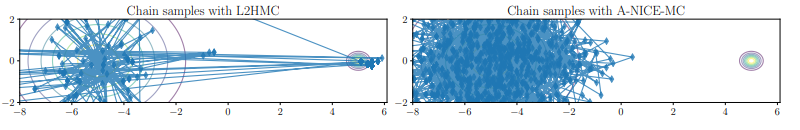
\includegraphics[width=\textwidth]{L2HMC-results.PNG}







\bibliographystyle{sysbio}
\bibliography{./L2HMC}

% **** THIS ENDS THE EXAMPLES. DON'T DELETE THE FOLLOWING LINE:

\end{document}

